%%%%%%%%%%%%%%%%%%%%%%%%%%%%%%%Section 2%%%%%%%%%%%%%%%%%%%%%%%%%%%%%%%%%%% 

\section{Hypothesis Testing}\label{sec:Hyp.Testing}
In a very broad sense, most of statistical inference is done through \textbf{hypothesis testing}: 
\begin{itemize}[noitemsep]
\item are the client's conjectures about their business situation compatible with the evidence provided by the data? 
\item is there a way to get a quantitative ruling in favour of one of several competing conjectures that relies on something other than gut feeling? 
\item can some of these conjectures be definitively eliminated?  \end{itemize}  Suppose that a researcher wants to determine if, as she believes, a new teaching method enables students to understand elementary statistical concepts better than the traditional lectures given in a university setting. \par She recruits  $N=80$ second-year students to test her claim. The students are randomly assigned to one of two groups: students in group $A$ are given the traditional lectures, whereas students in group $B$ are taught using the new teaching method. \par After three weeks, a short quiz is administered to the students in order to assess their understanding of statistical concepts -- Table~\ref{tab:SA1} summarises the results. 
\newl If we assume that both groups have similar background knowledge prior to being taught (which we attempt to do by randomising the group assignment), then the effectiveness of the teaching methods may be compared using two hypotheses: the \textbf{null hypothesis} $H_0$ and the \textbf{alternative}~$H_{\textrm{a}}$. Let $\mu_i$ represent the true performance of method~$i$. \newpage\noindent \textbf{One-sided testing}
     \begin{table}[t]
      \centering
     
         \begin{tabular}{c c c c}
         \hline
         \textbf{Group} & \textbf{Sample Size} & \textbf{Sample Mean} & \textbf{Sample Variance} \\
         \hline
         $A$ & $N_{A} = 40$ & $\bar{y}_{A} = 75.1$ & $S^{2}_{A}=6.7$ \\
         $B$ & $N_{B} = 40$ & $\bar{y}_{B} = 79.0$ & $S^{2}_{B}=5.5$ \\
        \hline
         \end{tabular}
     \caption[\small Summary of teaching method study example]{\small Summary of teaching method study example}
         \label{tab:SA1}\hrule
    
     \end{table}
     \afterpage{\FloatBarrier}
pits $$H_{0}: \mu_{A} \geq \mu_{B}\quad\mbox{against}\quad H_{\textrm{a}}: \mu_{A} < \mu_{B}$$ (or the reverse); in \textbf{two-sided testing}, we have $$H_{0}: \mu_{A} = \mu_{B}\quad\mbox{against}\quad H_{\textrm{a}}: \mu_{A} \neq \mu_{B}.$$ Intuitively, it would seem that testing for inequality of method seems a looser approach (i.e.\@ more general) than testing for the superiority of a specific method over the other. 
\newl Hypothesis testing can generate two types of error: 
\begin{itemize}[noitemsep]
\item we can mistakenly reject $H_0$ when it is, in fact, correct (\textbf{type I error}), or 
\item we can mistakenly accept $H_{0}$ when it is actually false (\textbf{type II error}). 
\end{itemize}In order to control the probability of making a type I error (called \textbf{significance level}, and denoted by $\alpha$), we usually let the hypothesis of interest be the alternative hypothesis.
\newl Since the researcher wants to claim that the new method is more effective than the traditional ones, then it is most appropriate for her to use one-sided hypothesis testing with $$H_{0}: \mu_{A} \geq \mu_{B} \quad\mbox{against}\quad H_{1}: \mu_{A} < \mu_{B};$$ The testing procedure is simple:
\begin{enumerate}[noitemsep]
\item calculate a \textbf{test statistic} under $H_0$;
\item reject $H_0$ in favour of $H_1$ if the test statistic falls in the \textbf{critical region} (also called \textbf{rejection region}) of an associated distribution (see Figure~\ref{fig:crit_reg}), and 
\item fail to reject $H_0$ otherwise, which is not quite the same thing as accepting it.
\end{enumerate}
Using the summary table above, we can test the researcher's claim by using the \textbf{two-sample $t$ test}. Assuming that variability in two groups are roughly the same, the test statistic is given by:
\begin{equation*}
    t_{0}=\frac{\bar{y}_{B}-\bar{y}_{A}}{S_{p}\sqrt{\frac{1}{N_{A}}+\frac{1}{N_{B}}}},
\end{equation*}
where the \textbf{pooled variance} $S^{2}_{p}$ is
\begin{equation*}
    S^{2}_{p}=\frac{(N_{A}-1)S^{2}_{A}+(N_{B}-1)S^{2}_{B}}{N_{A}+N_{B}-2}.
\end{equation*}
\begin{figure*}[t]
\centering
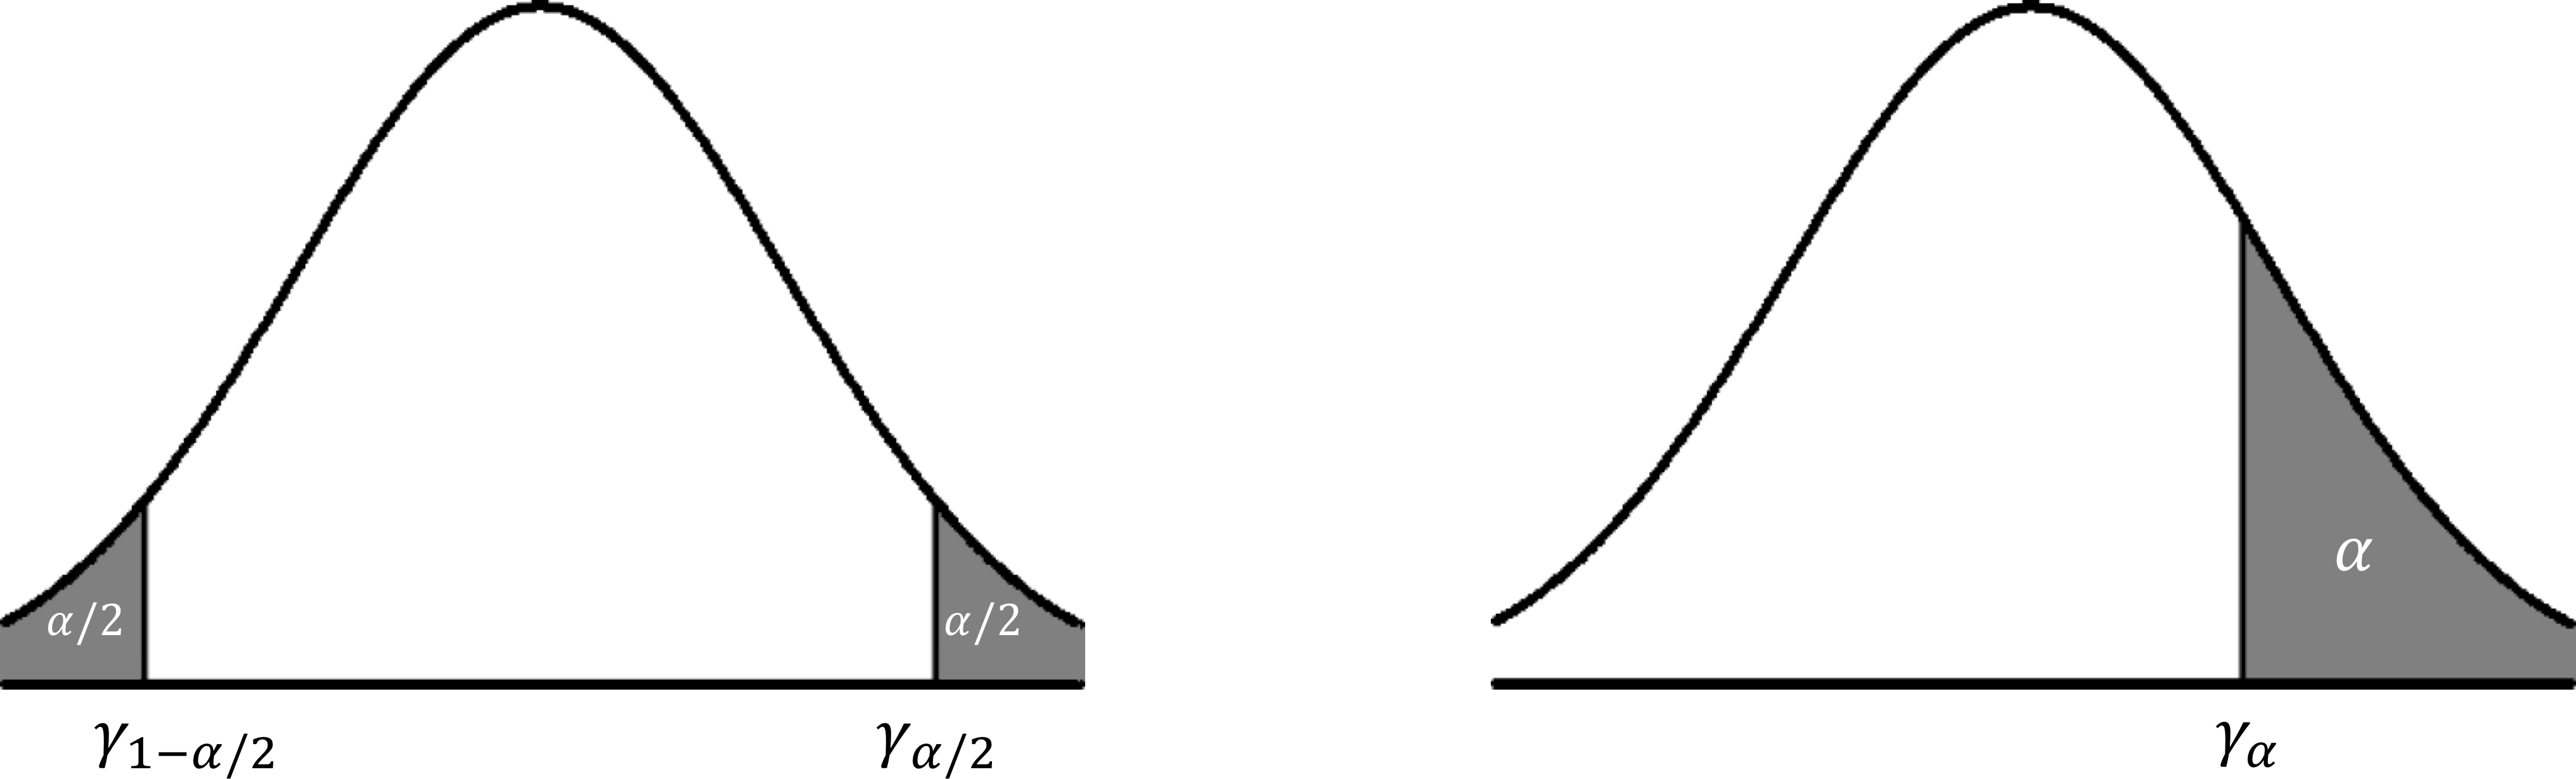
\includegraphics[width=0.8\textwidth]{Images/crit_reg.png}
\caption[\small Critical regions for hypothesis testing]{\small Critical regions for hypothesis testing at $\alpha$ (in grey); two-sided on the left, one-sided on the right; $\gamma_k$ represent the critical value for the given test and underlying distribution. }\label{fig:crit_reg}\hrule
\end{figure*}
\newpage\noindent In our example, the test statistic value is $t_{0} = 7.02$. To reject or accept the null hypothesis, we need to compare it against the \textbf{critical value} of the Student $T$ distribution with $N-2=78$ degrees of freedom at $\alpha=0.05$, which is \begin{equation*}t^*= t_{1-\alpha, N-2}=t_{0.95, 78}=1.665.\end{equation*} Since $t_{0} > t^*$ at $\alpha=0.05$, we have enough evidence to believe that the new teaching method is indeed more effective than the traditional methods, at $\alpha=0.05$.
\begin{center}
    \rule{0.25\textwidth}{.4pt}
\end{center} In general, the challenge is to recognise which test statistic to use and how it is distributed under $H_0$. Various scenarios have been explored in the literature (see \cite{SA_KNNL}, for instance); it could be useful  for analysts to be able to derive their own tests when the client's data does not meet the various assumptions. \par Ad-hoc solutions come at a price, however -- a fair number of clients (and reviewers), if they are familiar with statistical tests at all, do not understand how they are derived and thus only trust `tried, tested, and true' methods (this also applies to other fields of quantitative analysis). Custom approaches are likely to be treated with \textbf{suspicion}.   

\subsection{Questions to Ponder}
\begin{enumerate}[noitemsep,nolistsep]
    \item Distribution assumptions:
    \begin{itemize}[noitemsep]
        \item what distribution assumptions are we making by using a $t-$test?
        \item how can we verify them?
        \item if such assumptions are violated, what is our recourse?
    \end{itemize}
    \item Assumption of equal variance:
    \begin{itemize}[noitemsep]
        \item how can we verify the appropriateness of using pooled variance?
        \item if it is not appropriate, can we modify the test to overcome the problem?
    \end{itemize}
    \item One-sided vs. two-sided tests:
    \begin{itemize}[noitemsep]
        \item when is it appropriate to use a one-sided test, and when is it better to employ a two-sided test?
        \item are there drawbacks in using a two-sided test when a one-sided test would be indicated?
    \end{itemize}
\end{enumerate}

%%%%%%%%%%%%%%%%%%%%%%%%%%%%%%%Section 3%%%%%%%%%%%%%%%%%%%%%%%%%%%%%%%%%%% 
